A continuación se muestran las figuras obtenidas con el procedimiento obtenido anteriormente.

\begin{figure}[h!]
    \centering
    \begin{minipage}[t]{0.48\textwidth}
        \centering
        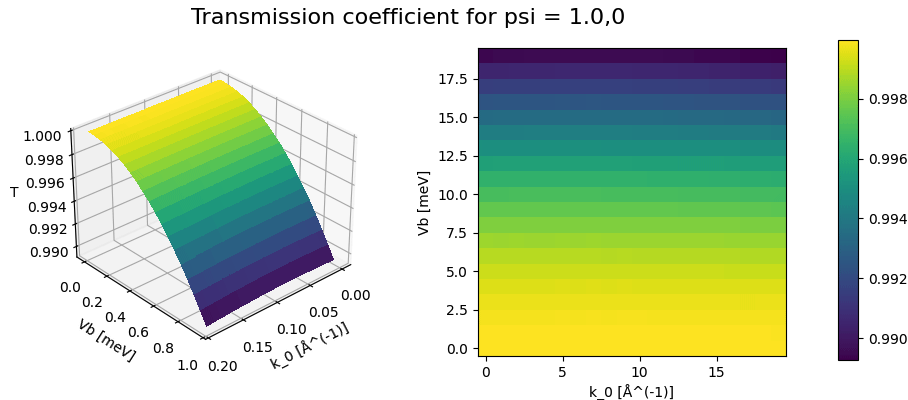
\includegraphics[width=\textwidth]{../assets/images/No-Rashba/TCoefficient(1.0,0)xalpha=0beta=0}
        \caption{figure}{
            Transmission coefficient ($T$) in pristine graphene with initial pseudospinor configuration $\xi = (1, 0)$, plotted against potential barrier height ($V_b$, in meV) and initial wave vector ($k_0$, in \AA$^{-1}$). The 3D plot and 2D heatmap show that transmission is largely independent of the initial wave vector but decreases noticeably as the barrier height increases, ranging from $1$ to approximately $0.990$.
        }
        \label{fig:noRashba}
    \end{minipage}
    \hfill
    \begin{minipage}[t]{0.48\textwidth}
        \centering
        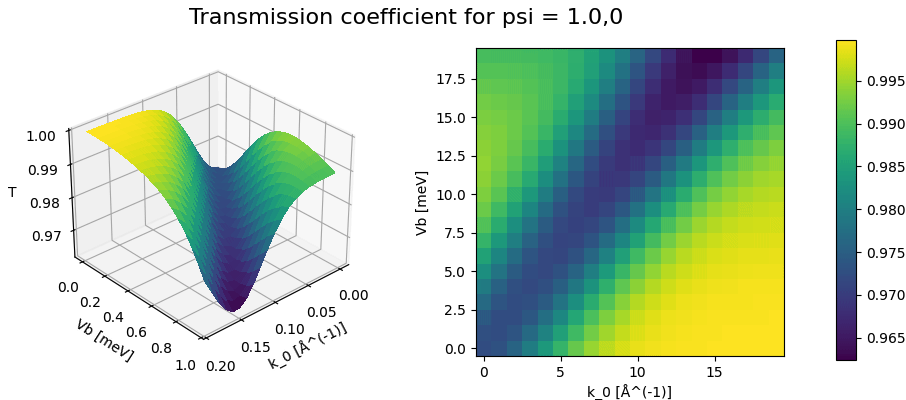
\includegraphics[width=\textwidth]{../assets/images/Rashba/TCoefficient(1.0,0)xalpha=0.2beta=-0.2}
        \caption{figure}{
            Coeficiente de transmisión ($T$) en función de la altura de la barrera de potencial ($V_b$) y el número de onda inicial ($k_0$) con una configuración inicial de pseudoespinor $\xi = (1, 0)$. La superficie 3D y el mapa de color 2D muestran una dependencia no monotónica de $T$ con respecto a $V_b$ y $k_0$, destacando la influencia del acoplamiento espín-órbita en la transmisión a través de la barrera.
        }
        \label{fig:rashba}
    \end{minipage}
\end{figure}

En las imágenes podemos notar ciertos aspectos interesantes, empezando con la fig.\ref{fig:noRashba}.
La imagen presenta dos gráficos que ilustran el coeficiente de transmisión ($T$) en función de $Vb$ (en meV) y $k_0$ (en \AA$^{-1}$) para un valor fijo de $\xi = (1, 0)$.
El gráfico de la izquierda es una visualización tridimensional donde $T$ está en el eje $z$, $Vb$ en el eje $x$ y $k_0$ en el eje $y$, con una escala de colores que varía desde morado oscuro (menor $T$) hasta amarillo brillante (mayor $T$).
El gráfico de la derecha es un mapa de calor bidimensional que ofrece una vista superior, con el eje $x$ representando $k_0$ y el eje $y$ representando $Vb$, usando el mismo mapa de colores que el gráfico 3D\@.
Ambos gráficos muestran que el coeficiente de transmisión generalmente se mantiene muy cerca de 1, indicando una alta transmisión.
Conforme aumenta $Vb$, $T$ tiende a disminuir, mientras que la dependencia respecto a $k_0$ es mínima.
En general, los gráficos demuestran cómo cambia $T$ con variaciones en $Vb$ y $k_0$, destacando una leve disminución de $T$ al aumentar $Vb$ y un cambio insignificante respecto a $k_0$.

Este resultado muestra una contradicción con lo que ya se especifíca en la literatura, en el grafeno se esperaría observar una transmisión total debido a las mismas propiedades del material\cite{horsell2008, Young2009}.

Estas diferencias observadas pueden atribuirse principalmente a los siguientes aspectos relacionados con nuestro método y condiciones de simulación:

\begin{itemize}
    \item Wave Packet Characteristics:
    Nuestra simulación utiliza un paquete de onda (GWP) compuesto por múltiples autoestados de momentum en lugar de considerar un único estado propio.
    Esta elección implica contribuciones simultáneas de varios estados, que potencialmente generan interferencias cuánticas afectando ligeramente el coeficiente de transmisión\cite{Staelens2021}.
    Este punto, resaltado por nuestra modelación dinámica en tiempo, marca una diferencia significativa respecto a los modelos teóricos ideales donde dichas interferencias no aparecen.

    Además, nuestra simulación contempla explícitamente la variable tiempo, algo poco frecuente en estudios teóricos previos ideales y estáticos.
    Investigar cómo estos aspectos dinámicos, como el tiempo de fase o el tiempo de túnel, afectan específicamente la transmisión observada es un objetivo importante propuesto para trabajos posteriores.

    \item Efectos de interferencia cuántica por dispersión del paquete en el tiempo:
    Como ha sido sugerido por la literatura\cite{MolgadoMex2018}, al evolucionar temporalmente un paquete de onda gaussiano suficientemente ancho, este se dispersa espacialmente de tal forma que diferentes partes del mismo interactúan simultáneamente con la barrera, causando interferencias internas consigo mismas.
    Tal interferencia es una posible causa adicional de las fluctuaciones en la transmisión observada en nuestros resultados numéricos.
\end{itemize}

Estos puntos explican las diferencias encontradas claramente desde una perspectiva metodológica y vinculan nuestros resultados numéricos respecto a la predicción teórica mencionada en los estudios previos.
Esto no solo aclara la aparente contradicción, sino que también permite reforzar claramente el vínculo entre nuestros resultados específicos y el objetivo principal de analizar efectos dinámicos y propiedades que surgen al emplear paquetes de onda Gaussianos en simulaciones de tunneling cuántico en sistemas basados en grafeno.

Por otro lado, tenemos la transmisión bajo presencia de SOIR (Fig.\ref{fig:rashba}).

Se observa una correlación entre las variables: generalmente, a mayor altura de la barrera de potencial ($Vb$) y mayor número de onda inicial ($k_0$), se espera una menor transmisión.
Sin embargo, la interacción espín-órbita introduce un comportamiento más complejo.
A medida que $k_0$ aumenta y $Vb$ disminuye, la transmisión se acerca a 1, indicando una mayor probabilidad de tunelamiento cuántico debido a la SOIR\@.

Aunque la variación en el coeficiente de transmisión es pequeña (del orden de $10^{-2}$), es significativa y atribuible a la interacción SOIR. Los electrones, con sus diferentes componentes de pseudoespín, interactúan, y esta interacción se ve afectada por el número de onda inicial del paquete de ondas gaussiano (GWP), como se observó en estudios previos\cite{Serna2019}.
Por lo tanto, la SOIR modula la interacción, lo que a su vez causa las fluctuaciones observadas en el coeficiente de transmisión.

Es importante destacar aquí que la obtención analítica del vector corriente (ec. \ref{eq:componentes}) ha sido determinante para interpretar los resultados obtenidos numéricamente.
En particular, esta ecuación permite vincular explícitamente diferencias observadas en los coeficientes de transmisión con los componentes pseudoespinoriales y sus correlaciones cruzadas debido a la interacción Rashba.
Por lo tanto, este resultado no solo brinda claridad conceptual, sino que también sienta las bases para futuras investigaciones teóricas y experimentales sobre transporte spintrónico avanzado en grafeno.

Tras analizar exhaustivamente los resultados numéricos y discutir los aspectos particulares observados en los coeficientes de transmisión electrónica con y sin interacción Rashba, podemos sintetizar a continuación las principales conclusiones alcanzadas en este trabajo, resaltando sus implicaciones teóricas y tecnológicas, así como las perspectivas para futuros estudios y aplicaciones.
